% Poster get from https://github.com/victorsenam/tcc/blob/master/poster/main.tex

\documentclass[final]{beamer}
\usepackage[size=a1,orientation=portrait,scale=1.3]{beamerposter}

\usepackage[brazil]{babel}
\usepackage[utf8]{inputenc}
\usepackage[T1]{fontenc}
\usepackage{framed,graphicx,xcolor} % for shaded box
\usepackage{mathtools}%
\usepackage{tcolorbox} % Para criar bordas elegantes
\usepackage{graphicx}  % Para incluir imagens
\usepackage{caption}   % Para legendas personalizadas
\usepackage{tikz}
\usetikzlibrary{matrix,shapes,positioning,shadows,trees,patterns}

\usepackage[shortlabels]{enumitem}
\usepackage[numbers]{natbib}
\bibliographystyle{plainnat}
  \def\bibfont{\small}

\sloppy

%----------------------------------------------------------------------------------------
%	SHORTCUTS
%----------------------------------------------------------------------------------------
\newcommand{\B}[1]{\mathbb{#1}}
\newcommand{\Cl}[1]{\ensuremath{\mathcal{#1}}}

\newcommand{\sse}{\Leftrightarrow}
\newcommand{\so}{\Rightarrow}
\newcommand{\se}{\Leftarrow}
\newcommand{\rec}{\leftarrow}

\newcommand{\tdots}{\,.\,.\,}

%----------------------------------------------------------------------------------------
%	BEAMER STYLE
%----------------------------------------------------------------------------------------

\usetheme{poster}
\setbeamercolor{block title}{fg=dblue,bg=white}
\setbeamercolor{block body}{fg=black,bg=white}
\setbeamercolor{block alerted title}{fg=dblue,bg=gray!50}
\setbeamercolor{block alerted body}{fg=black,bg=gray!20}
\setbeamercolor{block prob}{fg=black,bg=white}
\setbeamertemplate{caption}[numbered]

%----------------------------------------------------------------------------------------
%	CUSTOM STYLING
%----------------------------------------------------------------------------------------

\newenvironment<>{prob}{
    \begin{beamercolorbox}[sep=1ex,center,dp={1ex}]{block prob}
    \textcolor{dblue}{\textbf{Problema:}}\itshape
}{\end{beamercolorbox}}

\newcommand\halfcol{\column{.46\textwidth}}
\newcommand\onethirdcol{\column{.31\textwidth}}

\newcommand{\Oh}{\mathrm{O}}

% ?????????
\usepackage{subcaption}

\newcommand*\bolinha[1]{\; \tikz[inner sep=.25ex]\node[circle,draw]{#1}; \;}

%----------------------------------------------------------------------------------------
%	POSTER
%----------------------------------------------------------------------------------------

\title{Rainbow Version of Dirac's Theorem: An Algorithmic Approach}
\author{
  \begin{tabular}{l} % Define uma tabela com alinhamento à esquerda
    Nathan Luiz Bezerra Martins \hspace{200pt} Orientadora: Yoshiko Wakabayashi\\
    Willian Miura Mori
  \end{tabular}
}
\institute{\vspace{10pt}Departamento de Ciência da Computação,\\
Instituto de Matemática e Estatística, Universidade de São Paulo}

\begin{document}
\begin{frame}[fragile]\centering
  \vspace{-40pt}
  \begin{columns}[T]

    % ----------------------------------------------------------------------------------------
    % PRIMEIRA COLUNA
    % ----------------------------------------------------------------------------------------
    \onethirdcol
    \begin{alertblock}{Resumo}
      Dada uma coleção $G = {G_1, G_2, \ldots, G_n}$ de grafos de ordem $n$, definidos 
      sobre o mesmo conjunto de vértices e que satisfazem a condição de Dirac para cada 
      $G_i$, existe um $G$-transversal que forma um circuito hamiltoniano, também conhecido
      como Circuito Hamiltoniano Rainbow. Neste trabalho, desenvolvemos um 
      algoritmo eficiente que encontra um Circuito Hamiltoniano Rainbow. Fizemos implementações
      tanto em \texttt{C++} quanto em \texttt{Python} e realizamos testes de desempenho para comparar as duas versões.
      Utilizamos a biblioteca \texttt{manim} para fazer uma animação gráfica do algoritmo.
    \end{alertblock}

    \begin{block}{Conceitos básicos}
        \textbf{Definições principais:}
        \begin{itemize}
          \item Um grafo simples é um grafo não direcionado sem laços e sem arestas múltiplas.
          \item Um \textbf{ciclo hamiltoniano} de $G$ é um ciclo que visita cada vértice de $G$ exatamente uma vez.
          \item $\delta(G)$ é o grau mínimo de um vértice em $G$.
        \end{itemize}
        \vspace{0.5em}
        \textbf{Teorema de Dirac (\cite{dirac1952}):}
        Se um grafo simples $G$ com $n$ vértices tem grau mínimo $\delta(G) \geq \frac{n}{2}$, então $G$ contém um ciclo hamiltoniano.
    \end{block}

    \begin{block}{Versões Rainbow de problemas clássicos}
      \textbf{Definição:}

      A versão rainbow de um problema na teoria dos grafos é uma variação 
      que adiciona a restrição de cores à solução desejada. Nesse contexto, o termo rainbow (arco-íris) refere-se a estruturas em um grafo que utilizam 
      elementos provenientes de diferentes subconjuntos, ou arestas com diferentes rótulos ou cores, 
      garantindo que não haja repetições.
      \vspace{1em}

      \textbf{Teorema de Dirac (\textit{Versão Rainbow}):}

      Dada uma coleção $G = {G_1, G_2, \ldots, G_n}$ de grafos de ordem $n$, definidos
      sobre o mesmo conjunto de vértices e que satisfazem a condição de Dirac para cada
      $G_i$, existe um $G$-transversal que forma um circuito hamiltoniano, também conhecido
      como Circuito Hamiltoniano Rainbow.
      Cada grafo $G_i$ pode ser enxergado como se suas arestas fossem coloridas com a cor $i$.
      
      \begin{center}
        \begin{tcolorbox}[
            colframe=black,        % Border color
            colback=white,         % Background color
            coltitle=black,        % Title color (used for caption)
            width=0.6\textwidth,   % Box width, 60% of the text width
            boxrule=0.5mm,         % Border thickness
            arc=4mm,               % Rounded corners
            outer arc=1mm,         % Outer corner rounding
        ]
            \centering
            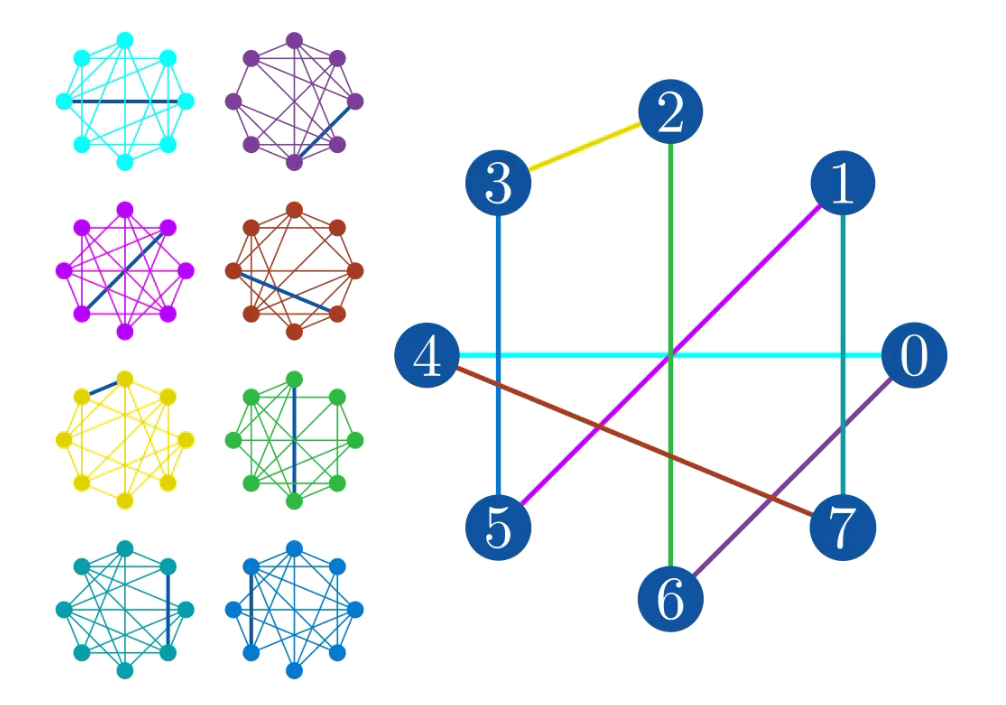
\includegraphics[width=\textwidth]{logos/dirac_rainbow.png}
            \captionof{figure}{Exemplo de um Circuito Hamiltoniano Rainbow para uma coleção de grafos com 8 vértices.}
        \end{tcolorbox}
      \end{center}

      \vspace{1em}
      \textbf{Mais exemplos clássicos:}
      \begin{itemize}
        \item \textbf{Floresta Geradora Mínima Rainbow:} Dado um grafo $G$ e uma coleção de cores, encontre uma floresta geradora mínima que utilize exatamente uma aresta de cada cor.
        \item \textbf{Emparelhamento Perfeito Rainbow:} Dado um grafo bipartido $G$ e uma coleção de cores, encontre um emparelhamento perfeito que utilize exatamente uma aresta de cada cor.
      \end{itemize}


    \end{block}

    % ----------------------------------------------------------------------------------------
    % SEGUNDA COLUNA
    % ----------------------------------------------------------------------------------------
    \onethirdcol

    \begin{exampleblock}


      As link-cut trees fornecem a seguinte interface:

      \definecolor{shadecolor}{rgb}{0.93, 0.80, 0.82} % pale pink
      \begin{shaded}
        \begin{itemize}
          \item[$\bullet$] \textbf{\texttt{make\_root(u)}}: enraíza no vértice $u$ a árvore que o contém
          \item[$\bullet$] \textbf{\texttt{link(u, v, w)}}: dado que os vértices $u$ e $v$ estão em árvores separadas, transforma $v$ em raiz de sua árvore e o liga como filho de $u$, colocando peso $w$ na nova aresta criada
          \item[$\bullet$] \textbf{\texttt{cut(u, v)}}: retira da floresta a aresta com pontas em $u$ e $v$, quebrando a árvore que continha estes vértices em duas novas árvores
          \item[$\bullet$] \textbf{\texttt{is\_connected(u, v)}}: retorna \texttt{verdadeiro} caso $u$ e $v$ pertençam à mesma árvore, \texttt{falso} caso contrário
          \item[$\bullet$] \textbf{\texttt{maximum\_edge(u, v)}}: retorna o peso máximo de uma aresta no caminho entre os vértices $u$ e $v$
        \end{itemize}
      \end{shaded}

      Todas essas operações consomem tempo $\Oh(\log n)$ amortizado, onde $n$ é o número de vértices na floresta.

    \end{exampleblock}

    \begin{block}{Union-Find retroativo}

      O union-find é uma estrutura de dados utilizada para manter uma \textbf{coleção de conjuntos disjuntos}, isto é, conjuntos que não se intersectam.

      \bigskip
      \begin{figure}[h!]
        \captionsetup{justification=centering}
        \centering
        \begin{subfigure}{\textwidth}
          \centering
          \begin{tikzpicture}[
              no/.style={shape=circle, minimum size=1cm},
              scale=1.5, transform shape
            ]
            \node[no] (a) at (4,0) {a};
            \node[no] (x) at (5,0) {};
            \node[no] (b) at (6,0) {b};
            \node[no] (y) at (7,0) {};
            \node[no] (c) at (8,0) {c};
            \node[no] (z) at (9,0) {};
            \node[no] (d) at (10,0) {d};

            \draw ($(x)$) ellipse ({1.7cm} and {.7cm});
            \draw ($(c)$) ellipse ({.7cm} and {.7cm});
            \draw ($(d)$) ellipse ({.7cm} and {.7cm});
          \end{tikzpicture}
          \bigskip
        \end{subfigure}
        \begin{subfigure}{\textwidth}
          \centering
          \begin{tikzpicture}[
              no/.style={shape=circle, minimum size=1cm},
              scale=1.5, transform shape
            ]
            \node[no] (a) at (4,0) {a};
            \node[no] (x) at (5,0) {};
            \node[no] (b) at (6,0) {b};
            \node[no] (y) at (7,0) {};
            \node[no] (c) at (8,0) {c};
            \node[no] (z) at (9,0) {};
            \node[no] (d) at (10,0) {d};

            \draw ($(x)$) ellipse ({1.7cm} and {.7cm});
            \draw ($(z)$) ellipse ({1.7cm} and {.7cm});
          \end{tikzpicture}
          \bigskip
        \end{subfigure}
        \begin{subfigure}{\textwidth}
          \centering
          \begin{tikzpicture}[
              no/.style={shape=circle, minimum size=1cm},
              scale=1.5, transform shape
            ]
            \node[no] (a) at (4,0) {a};
            \node[no] (x) at (5,0) {};
            \node[no] (b) at (6,0) {b};
            \node[no] (y) at (7,0) {};
            \node[no] (c) at (8,0) {c};
            \node[no] (z) at (9,0) {};
            \node[no] (d) at (10,0) {d};

            \draw ($(y)$) ellipse ({3.7cm} and {.7cm});
          \end{tikzpicture}
          \bigskip
        \end{subfigure}
        \begin{subfigure}{\textwidth}
          \centering
          \begin{tikzpicture}[
              no/.style={shape=circle, minimum size=1cm},
              scale=1.5, transform shape
            ]
            \node[no] (a) at (4,0) {a};
            \node[no] (x) at (5,0) {};
            \node[no] (b) at (6,0) {b};
            \node[no] (y) at (7,0) {};
            \node[no] (c) at (8,0) {c};
            \node[no] (z) at (9,0) {};
            \node[no] (d) at (10,0) {d};

            \draw ($(b)$) ellipse ({2.8cm} and {.7cm});
            \draw ($(d)$) ellipse ({.7cm} and {.7cm});
          \end{tikzpicture}
        \end{subfigure}
        \caption{Representação dos conjuntos com os elementos $\{a,b,c,d\}$ após a seguinte sequência de operações: \texttt{create\_union(a, b, 2)}, \texttt{create\_union(c, d, 3)}, \texttt{create\_union(b, c, 4)} e \texttt{delete\_union(3)}. Cada linha mostra o estado atual da coleção imediatamente após uma operação.}
        \label{fig:uf-sets}
      \end{figure}

      Na sua versão retroativa, implementamos as seguintes operações:

      \definecolor{shadecolor}{rgb}{0.93, 0.80, 0.82} % pale pink
      \begin{shaded}
        \begin{itemize}
          \item[$\bullet$] \textbf{\texttt{create\_union(a, b, t)}}: adiciona a união dos conjuntos que contém $a$ e $b$ no instante de tempo $t$
          \item[$\bullet$] \textbf{\texttt{same\_set(a, b, t)}}: consulta se dois elementos pertenciam ao mesmo conjunto no instante $t$
          \item[$\bullet$] \textbf{\texttt{delete\_union(t)}}: desfaz a união realizada em $t$
        \end{itemize}
      \end{shaded}


      Por exemplo, a Figura \ref{fig:uf-sets} mostra o estado de uma coleção de conjuntos disjuntos após quatro operações serem aplicadas. Antes da operação \texttt{delete\_union(3)}, as consultas \texttt{same\_set(a, b, 3)} e \texttt{same\_set(c, d, 3)} retornam \texttt{verdadeiro}. Por outro lado \texttt{same\_set(a, d, 3)} e \texttt{same\_set(c, d, 3)} retornam \texttt{falso} após a chamada da função \texttt{delete\_union(3)}.

      \definecolor{shadecolor}{rgb}{0.74, 0.83, 0.9} % pale blue
      \begin{shaded}
        \textbf{Ideia:} Fazer com que os elementos dos conjuntos sejam vértices na floresta mantida por uma link-cut tree, onde cada aresta representa uma operação de \texttt{union}. Assim, uma chamada \texttt{create\_union(a, b, 3)} cria uma aresta de valor $3$ entre os vértices $a$ e $b$. Da mesma forma, uma chamada \texttt{delete\_union(t)} simplesmente exclui a aresta criada no instante $t$. Para conferir se dois elementos $a$ e $b$, no instante de tempo $t$, estão em um mesmo conjunto, basta conferir se eles estão em uma mesma árvore e se o valor da maior aresta no caminho entre eles é menor ou igual a $t$, o que significa que todas as uniões já foram realizadas no instante consultado.
      \end{shaded}

    \end{block}




    % ----------------------------------------------------------------------------------------
    % TERCEIRA COLUNA
    % ----------------------------------------------------------------------------------------
    \onethirdcol

    \begin{block}{Implementação}

        A prova feita por \cite{Joos_2020} pode ser adaptada para um algoritmo construtivo, em que o estado é um caminho ou ciclo \textit{rainbow}, e incrementalmente aumentamos o tamanho desse caminho ou ciclo.

        A complexidade do algoritmo é da ordem de $\text{O}(n^3)$, em que $n$ é a ordem de $G$. Essa é complexidade é ótima, pois existem $\text{O}(n^3)$ arestas que devem ser consideradas no input.

        Para validar a corretude da implementação, foram gerados grafos que respeitavam a condição de Dirac com $n$ até $300$, e o código implementado devolvia o ciclo hamiltoniano \textit{rainbow}.

    \end{block}

    \begin{block}{Animação}

        Animação demonstrando o algoritmo foram feitas com a biblioteca \texttt{manim} (do canal de Youtube \texttt{3Blue1Brown}) em Python. Um exemplo está disponível no QR Code abaixo

        \begin{center}
            
\includegraphics[width=0.5\textwidth]{logos/qrcode.png} 
        \end{center}
    \end{block}

    \begin{block}{Referências}
      \bibliography{bibliografia.bib}
    \end{block}

  \end{columns}
\end{frame}
\end{document}
